\pdfoutput=1
%\documentclass[uplatex,dvipdfmx]{article}
\documentclass[pdftex]{article}



\usepackage{arxiv}

\usepackage[utf8]{inputenc}
\usepackage[T1]{fontenc}
\usepackage{hyperref}
\usepackage{url}
\usepackage{booktabs}
\usepackage{amsfonts} 
\usepackage{nicefrac}
\usepackage{microtype}
\usepackage{lipsum}
%\usepackage{graphicx}
\usepackage{natbib}
\usepackage{doi}
\usepackage{bm}
%\usepackage{lmodern}
\usepackage{kpfonts}
\usepackage{float}
\usepackage[pdftex]{graphicx}

\title{Optimization Calculation and LiNGAM}
%\date{July 14, 2021}

\author{ {\hspace{1mm}T .~Y}\\
	3D Engineering Solutions Dept.Research \& Development Group\\
	Neutral Ltd.
	\texttt{bccatfalcon@gmail.com} \\
	%% \AND
	%% Coauthor \\
	%% Affiliation \\
	%% Address \\
	%% \texttt{email} \\
	%% \And
	%% Coauthor \\
	%% Affiliation \\
	%% Address \\
	%% \texttt{email} \\
}


\renewcommand{\headeright}{Technical Report}
\renewcommand{\undertitle}{Technical Report}

%%% Add PDF metadata to help others organize their library
%%% Once the PDF is generated, you can check the metadata with
%%% $ pdfinfo template.pdf
\hypersetup{
	pdftitle={optimization calculation in the presence of unobserved latent common variables},
	pdfsubject={stat.ML, stat.CO},
	pdfauthor={Tatsuhiko .~Yamato},
	pdfkeywords={Causal search, Unobserved confounding,non-Gaussianity},
}

\begin{document}
\maketitle

\begin{abstract}
In recent years, as mechanisms such as \textbf{IoT}, \textbf{DX}, and \textbf{AI} have been introduced, the need for these technologies has increased.
More than that, however, there is a need to identify the root causes of problem occurrences and elucidate their mechanisms. One of the major obstacles is the assumption that there are no unobserved potential common causes.
The assumption that there are no unobserved potential common causes is a major obstacle for LiNGAM \cite{shimizu2006linear} to produce results. Although there are several previous studies, this method proposes a way to solve this problem by using known methods together.

\end{abstract}


% keywords
\keywords{Causal search \and Unobserved confounding \and non-Gaussianity}


\section{Introduction}
 It is well known that statistical causal search (LiNGAM) cannot estimate the correct causal structure when there are unobserved latent common variables. This is not necessarily a problem with LiNGAM itself, since the absence of unobserved latent common variables is a condition for applying LiNGAM, but in practice, knowing all variables and having them as observed data is a major problem in practice.
LiNGAM is represented by the following equation. The matrix B represents the causal structure between the data. Since the data distribution is assumed to be non-Gaussian, if the data distribution is not Gaussian, and moreover linear, the causal structure can be represented by this equation.

\begin{equation}
\mathbf{x}_{\mathbf{i}}\mathbf{=}\sum_{\mathbf{k}\left( \mathbf{j} \right)\mathbf{< k(i)}}^{}{\mathbf{B}_{\mathbf{\text{ij}}}\mathbf{x}_{\mathbf{j}}}\mathbf{+}\mathbf{\varepsilon}_{\mathbf{i}}
\end{equation}

This assumes that the residuals  $\mathbf{\varepsilon}_{\mathbf{i}}$ are independent of each other.
This assumes that there are no unobserved latent common causes in the data. The model can be extended to the case where there are unobserved latent common causes as follows.

\begin{equation}
\mathbf{x}_{\mathbf{i}}\mathbf{=}\mathbf{\mu}_{\mathbf{i}}\mathbf{+}\sum_{\mathbf{k}\left( \mathbf{j} \right)\mathbf{< k(i)}}^{}{\mathbf{B}_{\mathbf{\text{ij}}}\mathbf{x}_{\mathbf{j}}}\mathbf{+}\sum_{\mathbf{l = 1\cdots L}}^{}{\mathbf{\lambda}_{\mathbf{\text{il}}}\mathbf{f}_{\mathbf{l}}}\mathbf{+}\mathbf{\varepsilon}_{\mathbf{i}}\mathbf{\text{\ \ \ \ \ \ \ }}
\end{equation}

The unobserved potential common factor $\mathbf{\text{il}}$ needs to be determined in some way. However, since the number of unobserved potential common factors, L, is also unknown to begin with, the number of potential common factors, L, must also be determined, which will be very difficult.
\clearpage

\par
Representative Previous Research
LvLiNGAM (Latent variable LiNGAM) (\cite{hoyer2008estimation}), Pairewise LvLiNGAM algorithm(\cite{entner2010discovering}) (\cite{tashiro2014parcelingam}) and LiNGAM Mixture Model (\cite{shimizu2014bayesian}) have been proposed.



\section{Overview of the proposed method}
\label{sec:Overview}
\begin{equation}
x = \bm{B^{(c)} (x - \mu^{(c)}) + \mu^{(c)} + e^{(c)}}
\end{equation}
\centerline{(\cite{shimizu2014bayesian})}

\begin{equation}
x_{j} = \sum_{k(j)<k(i)}B_{i,j}(x_{j} - \mu_{j}) + e_{i} + \mu_{i}
\end{equation}
Problem to be solved
The basic idea is to attribute the entire problem to the optimization problem, and to find the cause-effect relationship of the whole rather than from the parts.

The optimization conditions and parameters are
\begin{itemize}
	\item The regression model is correct (residuals are minimized).
	\item The distribution parameters of $\mu$ are obtained so that the amount of mutual information in the residuals is minimized as much as possible.
	\item If there is prior knowledge of the causal relationship, add a penalty F due to the prior knowledge.
	\item Use a simple and easy to maintain algorithm
\end{itemize}

The above two conditions are to satisfy the LiNGAM requirement. It is a requirement of LiNGAM that the independence of residuals is equivalent to the absence of unobserved common causes. And it means that the data can be explained as a linear model.

It can be solved as a constrained multi-objective optimization problem with prior knowledge penalty, where the distribution parameters of µ are obtained so that the residuals of each variable do not fall into local solutions independently, while increasing the accuracy of the regression model under this condition.

\subsection{Optimization}
Optimization minimizes the amount of residuals and mutual information.
This is a multi-objective optimization calculation.
Determine the distribution parameters of $\mathbf{\mu}$ so that the amount of mutual information between residuals is minimized as much as possible.

\begin{equation}
\mu = {\mathbf{\text{arg~min}}}\left\lbrack \mathbf{\max}\left( \mathbf{\max}\left( \mathbf{e}_{\mathbf{i}} \right)\mathbf{,}\mathbf{\max}\left( \iint_{}^{}{p\left( \mathbf{e}_{\mathbf{i}},\mathbf{e}_{\mathbf{j}} \right)\log}\left( \frac{p\left( \mathbf{e}_{\mathbf{i}},\mathbf{e}_{\mathbf{j}} \right)}{p\left( \mathbf{e}_{\mathbf{i}} \right)p\left( \mathbf{e}_{\mathbf{j}} \right)} \right)d\mathbf{e}_{\mathbf{i}}d\mathbf{e}_{\mathbf{j}} \right)\mathbf{\ } \right)\mathbf{+ \theta\ penaltyF} \right\rbrack
\end{equation}
$\textbf{penaltyF} $ is a function that is zero if the prior knowledge of the causal structure is satisfied, but can be greater than zero otherwise. $\theta$ is a positive, sufficiently large value.\footnote{$p(e_{i})$ is the probability density of $e_{i}$.}

\begin{equation}
\mu\ \sim\ Generalized\_ Gaussian(\beta,\rho,\widetilde{x}) \equiv \frac{\beta^{\frac{1}{2}}}{2\mathbf{\Gamma}(1 + \frac{1}{\rho})}\mathbf{\exp}\left( {- \beta}^{\frac{1}{2}}\left| x - \widetilde{x} \right|^{\rho} \right)
\end{equation}

\begin{figure}[H]
	\centering
	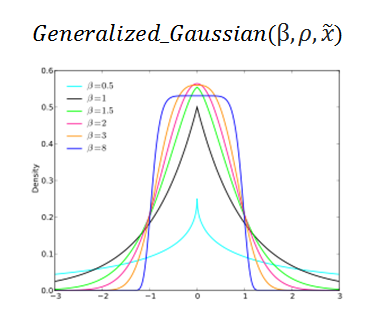
\includegraphics[width=5cm]{fig1.png}
	\caption{distribution}
\end{figure}

While improving the accuracy of the regression model, determine the parameters that determine the distribution of $\mu$ ($\beta,\rho,\widetilde{x}$) so that the residuals of each variable are independent, but do not fall into local solutions. The solution is obtained as a multi-objective optimization problem. 


\subsubsection{Loss computation}
Perform multi-objective optimization with the expanded Tchebyshev-scalarization function or the weighted average scalarization function.


\begin{equation}
\mathbf{\text{loss}}\mathbf{=}\mathbf{\max}\left(w1\ \text{independ}, \ w2\ \text{residual} \right) + \varepsilon\left( w1\ \text{independ} + \ \ w2\ \text{residual} \right)
\end{equation}
\centerline{\textbf{Expanded Tchebyshev-scalarization function}}

\begin{equation}
\mathbf{\text{loss}}\mathbf{=}w1\ \text{independ} + \ \ w2\ \text{residual}
\end{equation}
\centerline{\textbf{Weighted average scalarization function}}

$$w = \sqrt{best\_independ + best\_residual}$$
$$w1 = \frac{best\_independ}{w}$$ 
$$w2 =\frac{best\_residual}{w}$$
\leftline{$independ = maximum\ value\ of\ mutual\ information\ for\ each\ residual $}
\leftline{$residual = maximum\ absolute\ value\ of\ each\ residual$}
\leftline{$best\_ independ = maximum\ amount\ of\ mutual\ information\ between\ residuals\ at\ the\ best\ value\ of\ loss$}
\leftline{$best\_ residual = the\ maximum\ value\ of\ residuals\ at\ the\ best\ value\ of\ loss $}
\leftline{$\varepsilon = 0.0001$}

This optimization minimizes the residuals and the amount of mutual information, but in most cases the magnitudes of the maximum absolute values of the residuals and the amount of mutual information are quite different. However, in most cases, the magnitude of the maximum absolute value of the residuals and the magnitude of the mutual information are quite different. If the calculation of multi-objective optimization is performed as it is, only one of them may be minimized numerically. In this experiment, we found that both can be minimized by normalizing the maximum absolute value of the residuals used in the loss calculation and the maximum absolute value of the mutual information.
Normalization means to set the maximum absolute value of the residuals and the maximum absolute value of the mutual information calculated in the first evaluation of the optimization calculation to 1.0.
In our experiments, we found that it was not necessary to normalize the mutual information.

\section{experiment}
\label{sec:others}
The data used in the experiment is artificial data and unobserved conditions are created by excluding common cause variables.
The experiment generates the $\mu$ from a generalized Gaussian distribution \ref{distribution} and estimates the causal structure with LiNGAM. From this structure, we can calculate the residuals and mutual information for each variable.
Using this, we can search for $\mu$ until the residuals and mutual information are minimized.

In our experiments, we used the \textbf{Probabilistic} \textbf{Meta}-\textbf{Algorithm (SA) }to perform the calculations.
\begin{figure}[H]
	\centering
	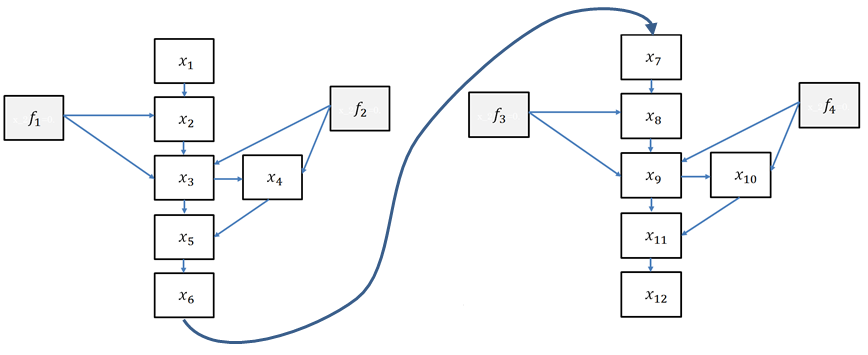
\includegraphics[width=10cm]{fig2.png}
	\caption{example causal structure}
	\label{fig2}
\end{figure}

For example, we created 19 cases of data as shown in \ref{fig2}.
$f_{1},f_{2},f_{3},f_{4}$ are the confounding variables.
By not including these variables in the data, we generate data with unobserved common causes.
\par
error term $e_{i}$ was set by a uniformly distributed random number.
\par
\leftline{$x_{1} = e_{1}$}
\leftline{$x_{2} = 0.4x_{1} + 0.8f_{1} + e_{2}$}
\leftline{$x_{3} = 0.3x_{2} + 0.7f_{1} + 0.7f_{2} + e_{3}$}
\leftline{$x_{4} = 0.2x_{3} + 0.8f_{2} + e_{4}$}
\leftline{$x_{5} = 0.5x_{3} + 0.5x_{4} + e_{5}$}
\leftline{$x_{6} = 0.5x_{5} +  e_{6}$}
\par
\leftline{$x_{7} = 0.5x_{6} +  e_{7}$}
\leftline{$x_{8} = 0.4x_{7} + 0.8f_{3} + e_{8}$}
\leftline{$x_{9} = 0.3x_{8} + 0.7f_{3} + 0.7f_{4} + e_{9}$}
\leftline{$x_{10} = 0.2x_{9} + 0.8f_{4} + e_{10}$}
\leftline{$x_{11} = 0.5x_{9} + 0.5x_{10} + e_{11}$}
\leftline{$x_{12} = 0.5x_{11} +  e_{12}$}

\subsection{Experimental results}
In LiNGAM, we got 30\% of the total causal direction wrong.(\ref{fig3})
\par
Our proposed method got all causal directions correct.(\ref{fig4})
\begin{figure}[H]
	\centering
	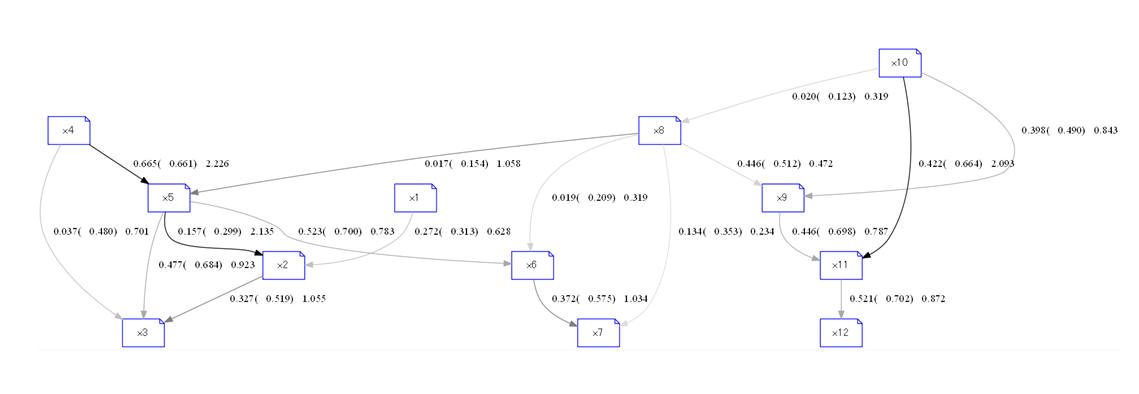
\includegraphics[width=15cm]{fig3.png}
	\caption{ICA LiNGAM}
	\label{fig3}
\end{figure}

\begin{figure}[H]
	\centering
	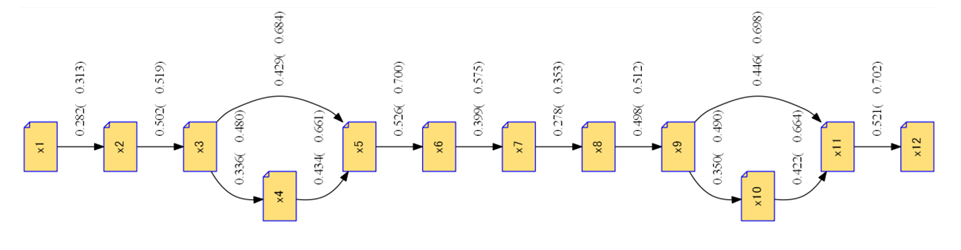
\includegraphics[width=15cm]{fig4.png}
	\caption{Our method}
	\label{fig4}
\end{figure}

\centerline{\textbf{results} \textbf{of} \textbf{the} \textbf{experiment} \textbf{for} \textbf{19 cases.}}


\begin{table}[H]
\caption{ 19 cases}
\begin{tabular}{l|l|l|l|}
\cline{2-4}
                                                                    & \textbf{ICA-LiNGAM} & \textbf{Our} & \textbf{Direct-LiNGAM} \\ \hline
\multicolumn{1}{|l|}{\textbf{Average}}                              & 84\%                & 100\%        & 85\%                   \\ \hline
\multicolumn{1}{|l|}{\textbf{Data without unobserved common cause}} & 96\%                & 100\%        & 100\%                  \\ \hline
\multicolumn{1}{|l|}{\textbf{Data with unobserved common cause}}    & 75\%                & 100\%        & 74\%                   \\ \hline
\end{tabular}
\label{tab:table1}
\end{table}
ICA-LiNGAM (\cite{shimizu2006linear}) , Direct-LiNGAM (\cite{shimizu2011directlingam}) , 
Even in the absence of unobserved data, the independence of the residuals and the residuals is corrected by optimization to create a more accurate linear model.\ref{fig5}



\begin{figure}[H]
	\centering
	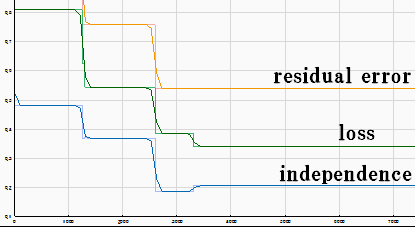
\includegraphics[width=5cm]{fig5.png}
	\caption{Optimization calculation}
	\label{fig5}
\end{figure}

\section{Discussion}
The advantage of this method is that it can be combined with existing computational techniques to build a highly maintainable system in a short period of time, and that there are few parameters that need to be adjusted.
The only parameter that needs to be adjusted is the maximum number of optimization iterations, which needs to be set by the user, but in most cases it converges after about 10000 iterations.

We also found a few problems.
The computation time is slow. In particular, when the number of variables exceeds 30, it can take a day to complete the calculation. We believe that this can be overcome by using GPU acceleration and parallelization well.
The biggest challenge is the possibility of computing the wrong path when the contribution of unobserved potential common variables is very large. Experiments have not included cases with very large impacts, but perhaps this should be assumed to be a realistic problem.
Another problem is that LiNGAM assumes continuous data, so it cannot be applied to discontinuous sensor data.
In this experiment, we used artificial data, but we would like to apply it to real-world data as well to clarify the scope of application and improve it if possible.

\section{Acknowledgments}
The style file used to create the Tex in this paper is available at https://github.com/kourgeorge/arxiv-style.
I would like to thank George Kour for his help in interpreting the significance of the results of this study.

%\bibliographystyle{unsrtnat}
\bibliographystyle{plain}
\bibliography{references}  %%%  .bib file (using bibtex) 

\clearpage
\appendix
\section{Statistical Causality}
\subsection{LiNGAM Model (Linear Non-Gaussian Acyclic Model)}

Given n observed variables $x=\left\{ x_{1},x_{2},\cdots,x_{n}\right\}$, estimates which variables affect which variables and by how much (causality).

The $\epsilon=\left\{\epsilon_{1},\epsilon_{2},\cdots,\epsilon_{n}\right\}$ are unobserved variables that may have an impact on the observed variables, such as noise and other factors that cannot be directly observed.

Assumption 1 \par
$\epsilon=\left\{\epsilon_{1},\epsilon_{2},\cdots,\epsilon_{n}\right\}$ are independent of each other and follow a non-Gaussian continuous distribution.

Note: Assuming independence means that for each observed variable, there is no unobserved common cause.

Assumption 2 \par
Linearity
$$\mathbf{x} = \mathbf{\text{Bx}} + \mathbf{\varepsilon}$$

$$\begin{pmatrix}
x_{1} \\
x_{2} \\
 \vdots \\
x_{n} \\
\end{pmatrix} = \begin{pmatrix}
B_{11} & B_{12} & \cdots & B_{1n} \\
B_{21} & B_{22} & \cdots & B_{2n} \\
 \vdots & \vdots & \cdots & \vdots \\
B_{n1} & B_{n2} & \cdots & B_{nn} \\
\end{pmatrix}\begin{pmatrix}
x_{1} \\
x_{2} \\
 \vdots \\
x_{n} \\
\end{pmatrix} + \begin{pmatrix}
\epsilon_{1} \\
\epsilon_{2} \\
 \vdots \\
\epsilon_{n} \\
\end{pmatrix}$$
Hereafter, the above matrix B will be referred to as the acyclic directed graph matrix. \par

Assumption 3 \par
We assume acyclicity in the causality of each observed variable. This means that when we consider a causal graph, no matter which variable we start from and follow the relationship, we cannot come back to the original variable, so

$$\begin{pmatrix}
x_{1} \\
x_{2} \\
 \vdots \\
x_{n} \\
\end{pmatrix} = \begin{pmatrix}
0 & 0 & \cdots & 0 \\
B_{21} & 0 & \cdots & 0 \\
 \vdots & \vdots & \cdots & \vdots \\
B_{n1} & B_{n2} & \cdots & 0 \\
\end{pmatrix}\begin{pmatrix}
x_{1} \\
x_{2} \\
 \vdots \\
x_{n} \\
\end{pmatrix} + \begin{pmatrix}
\epsilon_{1} \\
\epsilon_{2} \\
 \vdots \\
\epsilon_{n} \\
\end{pmatrix}$$

$$x_{1} = \epsilon_{1}$$

$$x_{2} = {B_{21}x}_{1} + \epsilon_{2}$$

$$x_{i} = {B_{i1}x}_{1} + {{B_{i2}x}_{2} + {B_{i2}x}_{3} + \cdots + {B_{\text{ik}}x}_{k} + \epsilon}_{i}\ \ \ \ \ \ k < i$$

$$x_{n} = B_{n1}x_{1} + B_{n2}x_{2} + \cdots + \epsilon_{n}$$

$$x_{1} = \epsilon_{1}$$

$$x_{2} = {B_{21}x}_{1} + \epsilon_{2}$$
The non-zero components represent a measure of how much each observable affects the observables on the left-hand side.

\subsection{Calculation procedure for ICA-LiNGAM}
Calculating the Acyclic Directed Graph Matrix \par

irst, we need to find the $\epsilon=\left\{\epsilon_{1},\epsilon_{2},\cdots,\epsilon_{n}\right\}$ that is not directly observed.

$$\mathbf{x} = \mathbf{\text{Bx}} + \mathbf{\varepsilon}$$.

$$\mathbf{\varepsilon = x} - \mathbf{Bx \rightarrow \varepsilon =}\left( \mathbf{I - B}\right)\mathbf{x}$$

$$\mathbf{W \equiv}\left( \mathbf{I - B}\right)$$

$$\mathbf{\varepsilon = Wx}$$.

Estimate W here (can be calculated using FastICA, an estimation method for independent component analysis).

If we know the appropriate substitution matrix P and the appropriate matrix D of the scaling transformation, we can obtain the restoration matrix $$\mathbf{W}_{\mathbf{\text{ICA}}}$$ that can be calculated using the FastICA method of independent component analysis estimation.

$$\mathbf{W \cong}\mathbf{D}^{\mathbf{-1}}\mathbf{P}\mathbf{W}_{\mathbf{\text{ICA}}}$$.

The substitution matrix P rearranges the rows such that the absolute value of the diagonal component of the restoration matrix $\mathbf{W}_{\mathbf{\text{ICA}}}$ is maximized.

The scale transformation matrix D is $D = diag(\mathbf{P}\mathbf{W}_{\mathbf{\text{ICA}}}\mathbf{)}$

$$\text{diag}\begin{pmatrix}
X_{11} & X_{12} & \cdots & X_{1n} \\
X_{21} & X_{22} & \cdots & X_{2n} \\
 \vdots & \vdots & \cdots & \vdots \\
X_{n1} & X_{n2} & \cdots & X_{nn} \\
\end{pmatrix} \equiv \begin{pmatrix}
X_{11} & 0 & \cdots & 0 \\
0 & X_{22} & \cdots & 0 \\
 \vdots & \vdots & \cdots & \vdots \\
0 & 0 & \cdots & X_{nn} \\
\end{pmatrix}$$

$$\mathbf{B = I - W \cong I -}\mathbf{D}^{\mathbf{- 1}}\mathbf{P}\mathbf{W}_{\mathbf{\text{ICA}}}$$
This does not necessarily mean that the acyclic directed graph matrix B computed with this guarantees acyclicity. In other words, redundant causal relations appear, so we remove them. The proposed method is as follows.

Forcibly replace $n(n + 1)/2$ components of B with zero components in the order of decreasing absolute value.

Check if each row of B can be rearranged into a lower triangular matrix, and if not, replace the next smallest absolute value component with zero.



\end{document}

%%arxiv.sty
%%MIT License
%%
%%Copyright (c) 2020 George Kour
%%
%%Permission is hereby granted, free of charge, to any person obtaining a copy
%%of this software and associated documentation files (the "Software"), to deal
%%in the Software without restriction, including without limitation the rights
%%to use, copy, modify, merge, publish, distribute, sublicense, and/or sell
%%copies of the Software, and to permit persons to whom the Software is
%%furnished to do so, subject to the following conditions:
%%
%%The above copyright notice and this permission notice shall be included in all
%%copies or substantial portions of the Software.
%%
%%THE SOFTWARE IS PROVIDED "AS IS", WITHOUT WARRANTY OF ANY KIND, EXPRESS OR
%%IMPLIED, INCLUDING BUT NOT LIMITED TO THE WARRANTIES OF MERCHANTABILITY,
%%FITNESS FOR A PARTICULAR PURPOSE AND NONINFRINGEMENT. IN NO EVENT SHALL THE
%%AUTHORS OR COPYRIGHT HOLDERS BE LIABLE FOR ANY CLAIM, DAMAGES OR OTHER
%%LIABILITY, WHETHER IN AN ACTION OF CONTRACT, TORT OR OTHERWISE, ARISING FROM,
%%OUT OF OR IN CONNECTION WITH THE SOFTWARE OR THE USE OR OTHER DEALINGS IN THE
%%SOFTWARE.
